\documentclass[11pt]{beamer}
\usetheme{Rochester}
\usecolortheme{seagull}
\usepackage[utf8]{inputenc}
\usepackage[german]{babel}
\usepackage[T1]{fontenc}
\usepackage{amsmath}
\usepackage{amsfonts}
\usepackage{amssymb}
\usepackage{textpos}

\usepackage{media9}
\addmediapath{../movies/}

% add logo to the sections
\addtobeamertemplate{frametitle}{}{%
\begin{textblock*}{100mm}(.6\textwidth,-1.2cm)

\includegraphics[width=0.5\linewidth]{./logo_inf_fak.png}
\end{textblock*}}


\setbeamertemplate{footline}[frame number]

\author{Michael Größler | Martin Zettwitz}
\title{An interactive ray tracing system \\ based on Nvidia OptiX}
\date{14. Oktober 2015} 
%\setbeamercovered{transparent}  
%\subject{}


\begin{document}

\begin{frame}
\titlepage
\end{frame}

\begin{frame}
\frametitle{Inhalt} 
\tableofcontents
\end{frame}





\section{Wer sind wir?}
\begin{frame}
\frametitle{Wer sind wir?} 
\begin{center}
Michael Größler \\ {\small 5. Semester CV \\ groessle@st.ovgu.de} 
\parskip 24pt

Martin Zettwitz \\ {\small 5. Semester CV \\ martin.zettwitz@st.ovgu.de}
\end{center}
\end{frame}



\section{Ziel des Projekts}
\begin{frame}
\frametitle{Ziel des Projekts}
\begin{itemize} 
\item Projekt- und Programmiererfahrung erweitern
\item interaktives Ray Tracing entwickeln
\item sich mit verschiedenen BRDFs auseinandersetzen
\item mit Bestnote abschließen
\end{itemize}
\end{frame}



\section{Rendering Equation}
\begin{frame}[allowframebreaks]
\frametitle{Rendering Equation}
\begin{center} 
'THE RENDERING EQUATION' \\ by James T. Kajiya [KAJ86] 

\begin{equation}
L_o(x,\vec{\omega_o}) = L_e(x,\vec{\omega_o}) + \int_\Omega f_r(\vec{\omega_i},\vec{\omega_o}) \cdot \cos\theta \cdot L_i(x,\vec{\omega_i}) \cdot d\vec{\omega_i}\
\end{equation}

\framebreak
$
L_o(x,\vec{\omega_o}) = L_e(x,\vec{\omega_o}) + \int_\Omega f_r(\vec{\omega_i},\vec{\omega_o}) \cdot \cos\theta \cdot L_i(x,\vec{\omega_i}) \cdot d\vec{\omega_i}\
$
\parskip 12 pt

\begin{table}[h]
\begin{tabular}{| c | l |}
\hline
$L_o$ & out-going radiance\\ \hline
$L_e$ & self emission\\ \hline
$L_i$ & in-going radiance\\ \hline
$\vec{\omega_i}$ & incoming light direction\\ \hline
$\vec{\omega_o}$ & vector towards camera\\ \hline
$f_r$ & BRDF\\ \hline
$\Omega$ & Hemisphere over point x\\ \hline
$\cos\theta$ & angle between normal and $\vec{\omega_i}$\\ \hline
$x$ & point on surface\\ \hline
\end{tabular}
\end{table}

\framebreak

Unser Ansatz ohne Eigenemmision und zusätzlicher Reflexion (CG)

\begin{equation}
L_o(x,\vec{\omega_o}) = \delta L_i(x,\vec{\omega_r}) + (1- \delta) \sum_{i=1}^{k} f_r(\vec{\omega_i},\vec{\omega_o}) \cdot E
\end{equation}
\parskip 12pt

\begin{table}[H]
\begin{tabular}{| c | l |}
\hline
$\delta$ & reflection coefficient\\ \hline
$E$ & approximated irradiance\\ \hline
$I_o$ & light intensity of a point light (independent from $\vec{\omega_i}$)\\ \hline
\end{tabular}
\end{table}
\end{center}

\end{frame}



\section{BRDFs}
\begin{frame}
\frametitle{BRDFs}
\begin{itemize}
\item bi-directional distribution function
\item beschreibt Lichtverhalten auf Oberflächen
\item betrachtet Ein- und Ausfallvektor
\item unterteilt in diffusen($K_d$) und spekularen($K_s$) Anteil
\end{itemize}
\parskip 10pt

\begin{equation}
f_r = K_d + K_s
\end{equation}

\begin{table}[H]
\begin{tabular}{| c | l |}
\hline
$\vec{V}$ & ray from hit point to camera\\ \hline
$\vec{N}$ & normal on hit point\\ \hline
$\vec{L}$ & ray from hit point to light source\\ \hline
\end{tabular}
\end{table}

\end{frame}



\subsection{Lambert}
\begin{frame}
\frametitle{Lambert}
\begin{center}
\begin{itemize}
\item nach Lambert's Emissions Gesetz aus 'Photometria' von Johann Heinrich Lambert in 1760
\item einfachste Darstellung perfekt diffuser Oberflächen
\end{itemize}

\begin{equation}
K_d = \frac{1}{\pi}
\end{equation}

$K_s = 0$
\parskip 12pt

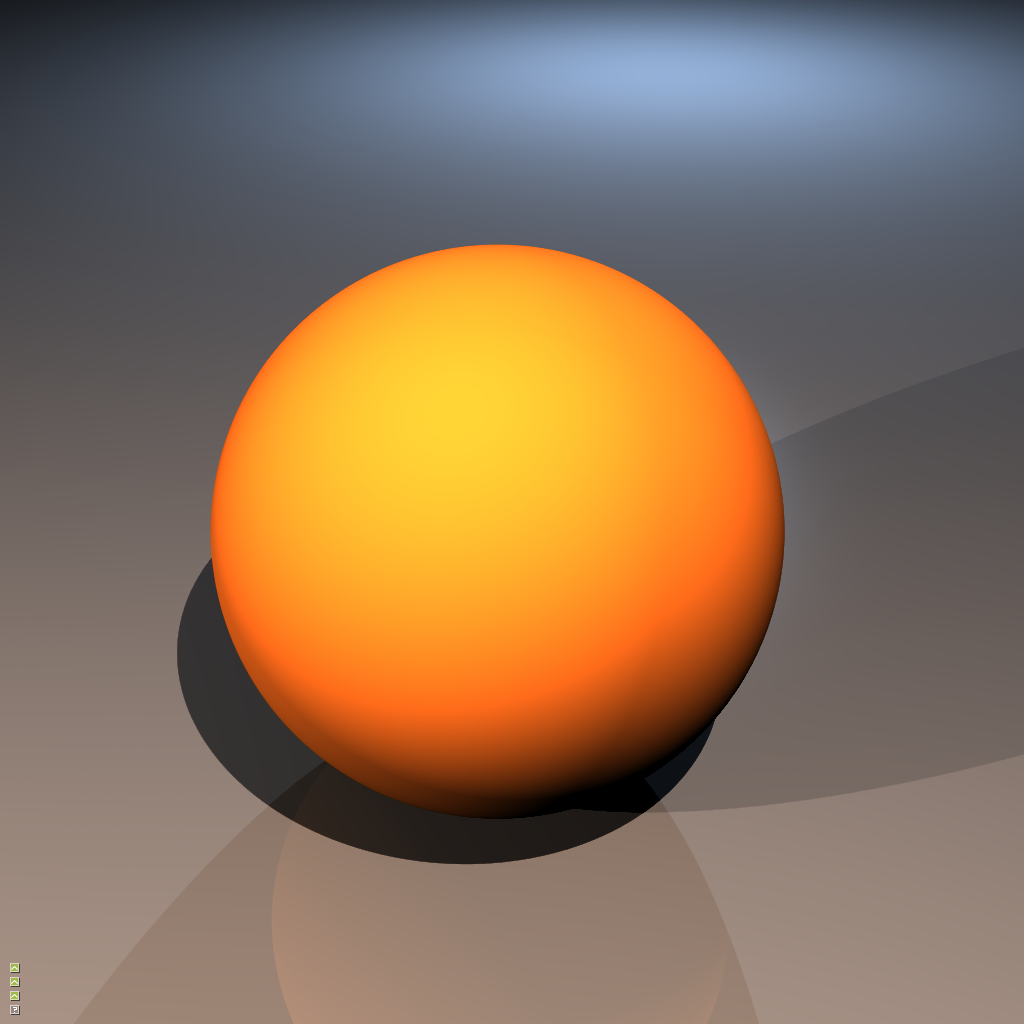
\includegraphics[width=0.2\linewidth]{../sopro/phong/phongdiff10}
\end{center}
\end{frame}



\subsection{Phong}
\begin{frame}[allowframebreaks]
\frametitle{Phong}

\begin{itemize}
\item nach [Pho75]
\item einfaches und erstes empirisches standard Modell für glänzende Oberflächen(Kunststoff)
\end{itemize}


\begin{equation}
K_d = \frac{\rho_d}{\pi}
\end{equation}
\begin{equation}
K_s = \rho_s \cdot \frac{s+2}{2\pi} \cdot cos^s\psi
\end{equation}

\begin{table}[H]
\begin{tabular}{| c | l |}
\hline
$\rho_d$ & Parameter : diffuse coefficient\\ \hline
$\rho_s$ & Parameter : specular coefficient\\ \hline
$s$ & Parameter : shiny exponent, controls roughness\\ \hline
$cos\psi$ & angle between outgoing and reflected ray\\ \hline
\end{tabular}
\end{table}

\framebreak
\begin{figure}[H]
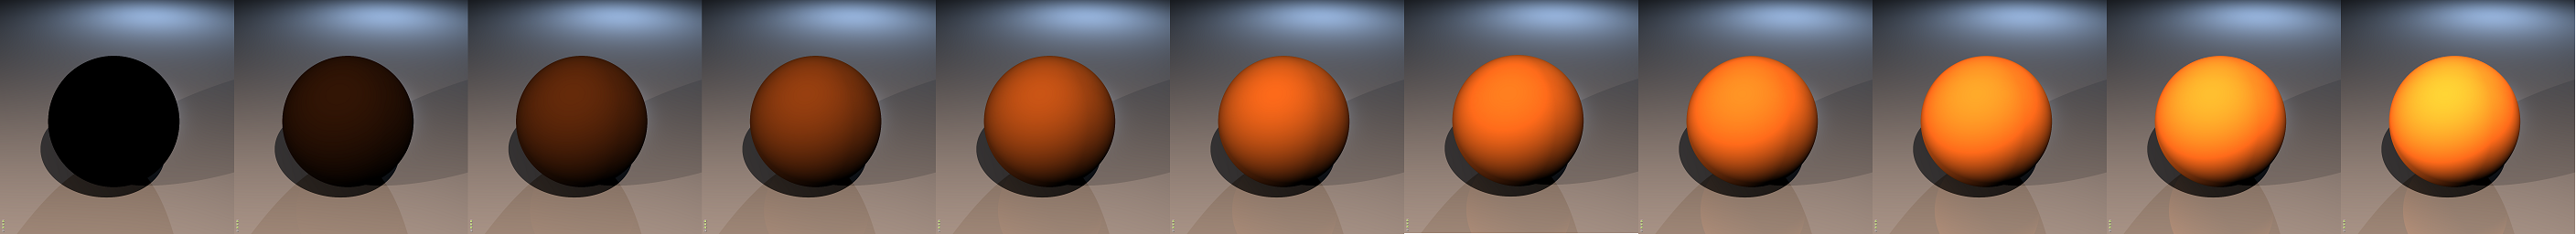
\includegraphics[width=\textwidth]{../phongdiffcomplete}
\caption{Parameter $\rho_d$ from $0.0$ to $1.0$}
\end{figure}

\begin{figure}[H]
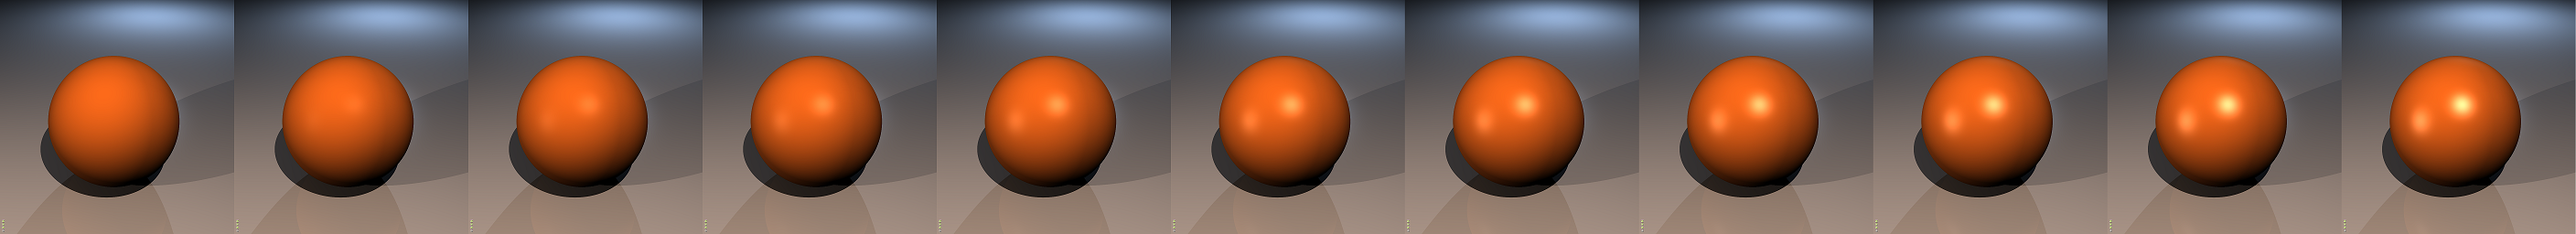
\includegraphics[width=\textwidth]{../phongspeccomplete}
\caption{Parameter $\rho_s$ from $0.0$ to $1.0$}
\end{figure}

\begin{figure}[H]
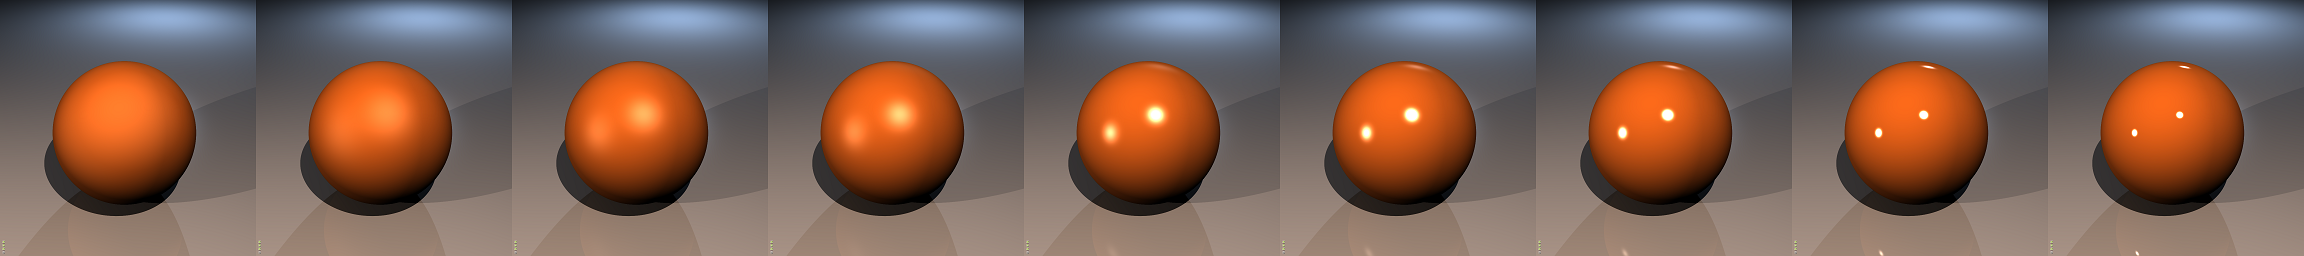
\includegraphics[width=\textwidth]{../phongshinecomplete}
\caption{Parameter $s$ from $1$ to $1000$}
\end{figure}

\begin{figure}[H]
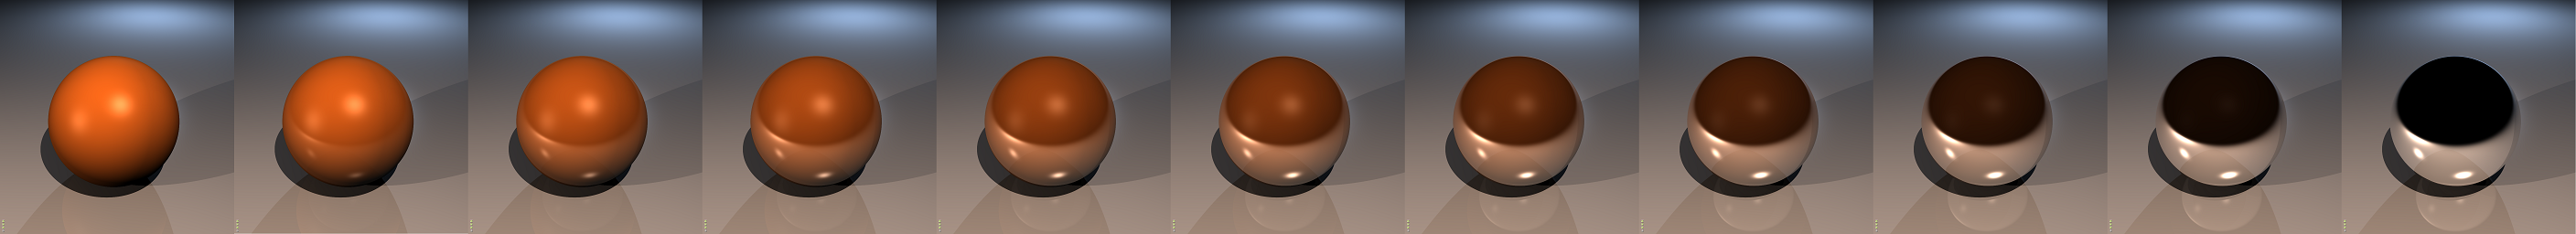
\includegraphics[width=\textwidth]{../phongreflcomplete}
\caption{Parameter $\delta$ from $0.0$ to $1.0$}
\end{figure}

\end{frame}



\subsection{Blinn Phong}
\begin{frame}[allowframebreaks]
\frametitle{Blinn Phong}
\begin{itemize}
\item nach [Bli77]
\item erweitert das standard Phong-Modell um den Halbvektor $\vec{H}$
\end{itemize}

\begin{equation}
K_d = \frac{\rho_d}{\pi}
\end{equation}
\begin{equation}
K_s = \rho_s \cdot \frac{s+8}{8\pi} \cdot cos^s\psi
\end{equation}

\begin{table}[H]
\begin{tabular}{| c | l |}
\hline
$\cos\psi$ & angle between outgoing ray and half vector $\vec{H}$\\ \hline
\end{tabular}
\end{table}
\begin{equation}
\vec{H} = \frac{\vec{L}+\vec{V}}{length(\vec{L}+\vec{V})}
\end{equation}

\begin{figure}[H]
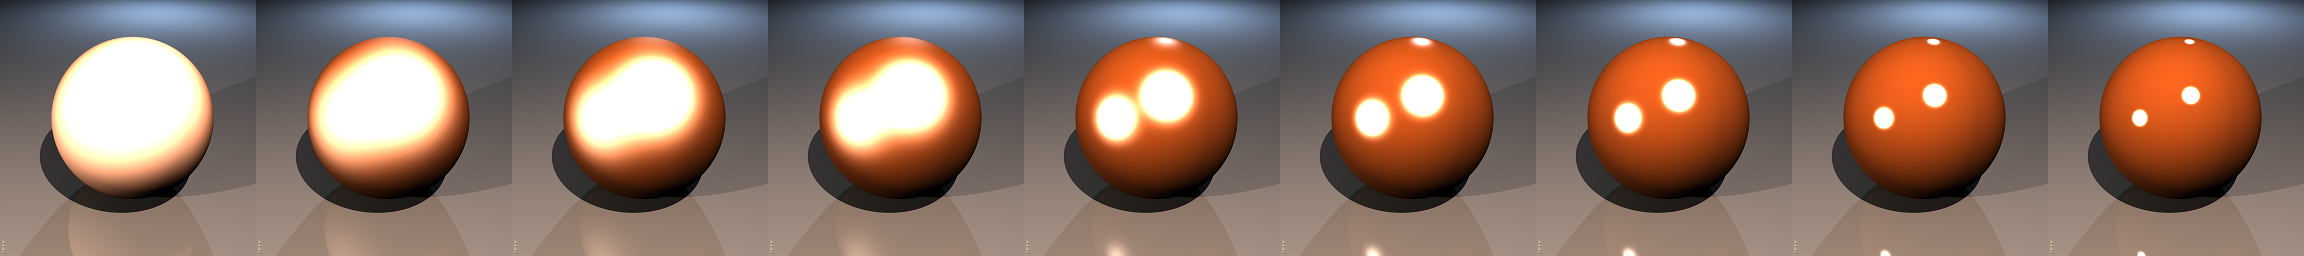
\includegraphics[width=\textwidth]{../blinnphongshinecomplete}
\caption{Parameter $s$ from $1$ to $1000$}
\end{figure}

\end{frame}



\subsection{Cook Torrance}
\begin{frame}[allowframebreaks]
\frametitle{Cook Torrance}

\begin{itemize}
\item basiert auf [CT82]
\item physikalisch basiertes Reflexionsmodell mit Microfacetten
\item simuliert isotrope metallische Oberflächen
\end{itemize}

\begin{equation}
K_d = \frac{\rho_d}{\pi}
\end{equation}
\begin{equation}
K_s =\rho_s \frac{D \cdot F \cdot G}{4(\vec{V} \cdot \vec{N})(\vec{N} \cdot \vec{L})}
\end{equation}

\begin{table}[H]
\begin{tabular}{| c | l |}
\hline
$D$ & Beckmann distribution\\ \hline
$F$ & Fresnel term\\ \hline
$G$ & Geometric attenuation (Torrance Sparrow)\\ \hline
\end{tabular}
\end{table}

\framebreak

Beckmann distribution:
\begin{equation}
D = \frac{e^{-\frac{tan^2(\alpha)}{m^2}}}{\pi \cdot m^2 \cdot cos^4(\alpha)}\label{eq:beckmann} , \alpha = arccos(\vec{N} \cdot \vec{H})
\end{equation}

Fresnel term, based on [Sch94]:
\begin{equation}
F = \delta + (1-\delta)(1-cos(\theta))^5 , \delta = \left(\frac{\eta - 1}{\eta+1}\right)^2
\end{equation}

Geometric attenuation:
\begin{equation}
G = min \left(1,\frac{2(\vec{H} \cdot \vec{N})(\vec{V} \cdot \vec{N})}{\vec{V} \cdot \vec{H}},\frac{2 (\vec{H} \cdot \vec{N})(\vec{L} \cdot \vec{N})}{\vec{V} \cdot \vec{H}}\right)
\end{equation}


\framebreak
\begin{table}[H]
\begin{tabular}{| c | l |}
\hline
$m$ & Parameter : controls roughness of surface\\ \hline
$\eta$  & Parameter : Fresnel factor(refractive index)\\ \hline
$\theta$  & Angle between $\vec{L}$ and $\vec{H}$\\ \hline
\end{tabular}
\end{table}
Gleichung \ref{eq:beckmann} wurde durch folgenden Substitution vereinfacht:
\begin{equation}
\frac{tan^2(\alpha)}{m^2} = \frac{1- cos^2(\alpha)}{cos^2(\alpha) \cdot m^2}
\end{equation}

\framebreak
\begin{figure}[H]
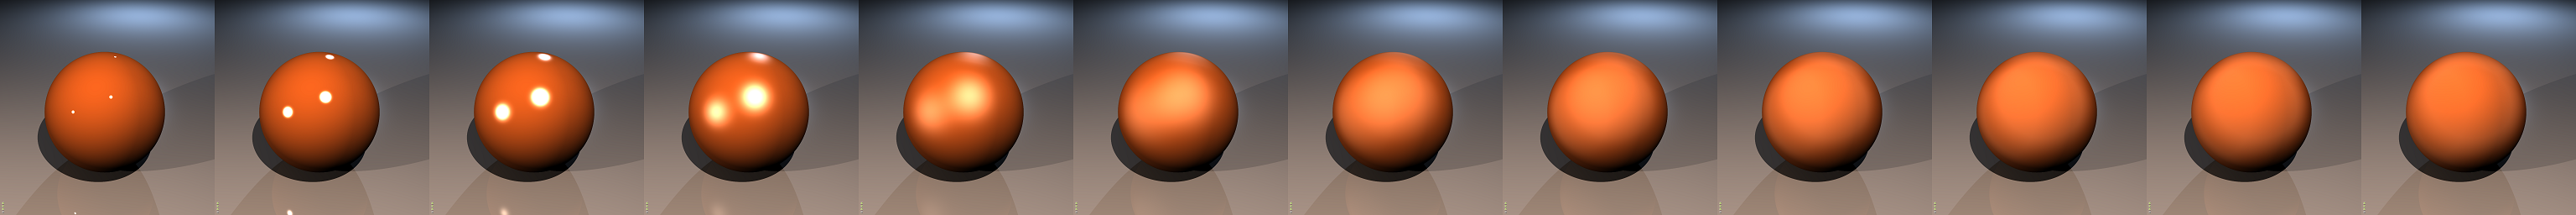
\includegraphics[width=\textwidth]{../ctroughcomplete.png}
\caption{Parameter $m$ from $0.01$ to $1.0$}
\end{figure}

\begin{figure}[H]
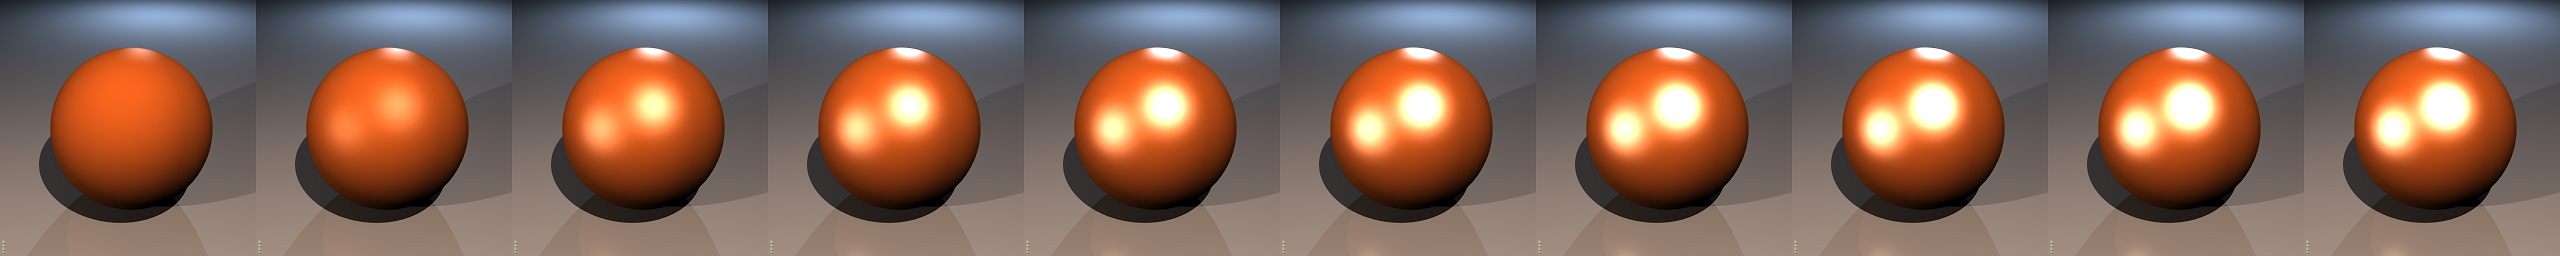
\includegraphics[width=\textwidth]{../ctfresnelcomplete.png}
\caption{Parameter $\eta$ from $1.0$ to $10.0$}
\end{figure}

\end{frame}



\subsection{Ward}
\begin{frame}[allowframebreaks]
\frametitle{Ward}
%TODO

\begin{itemize}
\item basierend auf [GMD10]
\item experimentelles, einfach zu berechnendes Modell
\item simuliert anisotrope metallische Oberflächen
\end{itemize}

\begin{equation}
K_d = \frac{\rho_d}{\pi}
\end{equation}

\begin{equation}
K_s = \frac{\rho_s}{4 \pi \alpha_x \alpha_y } 
\cdot e^
{
- \frac{(\frac{\vec{h} \cdot \vec{x}}{\alpha_x})+(\frac{\vec{h} \cdot \vec{y}}{\alpha_y})}
{(\vec{h} \cdot \vec{N})^2}
}
\cdot 
\frac{1}{4 (\vec{H} \cdot \vec{L})^2 (\vec{H} \cdot \vec{N})^4}
\end{equation}

\framebreak

\begin{table}[H]
\begin{tabular}{| c | l |}
\hline
$\alpha_x$ & Parameter : horizontal control of brush\\ \hline
$\alpha_y$ & Parameter : vertical control of brush \\ \hline
$\vec{h}$ & Half vector between $\vec{L}$ and $\vec{V}$ \\ \hline
$\vec{H}$ & Normalized half vector between $\vec{L}$ and $\vec{V}$ \\ \hline
$\vec{x}$ & Tangent Vector to $\vec{N}$ \\ \hline
$\vec{y}$ & Tangent Vector to $\vec{N}$, perpendicular to $\vec{x}$ \\ \hline
\end{tabular}
\end{table}

\framebreak

\begin{figure}[H]
\centering

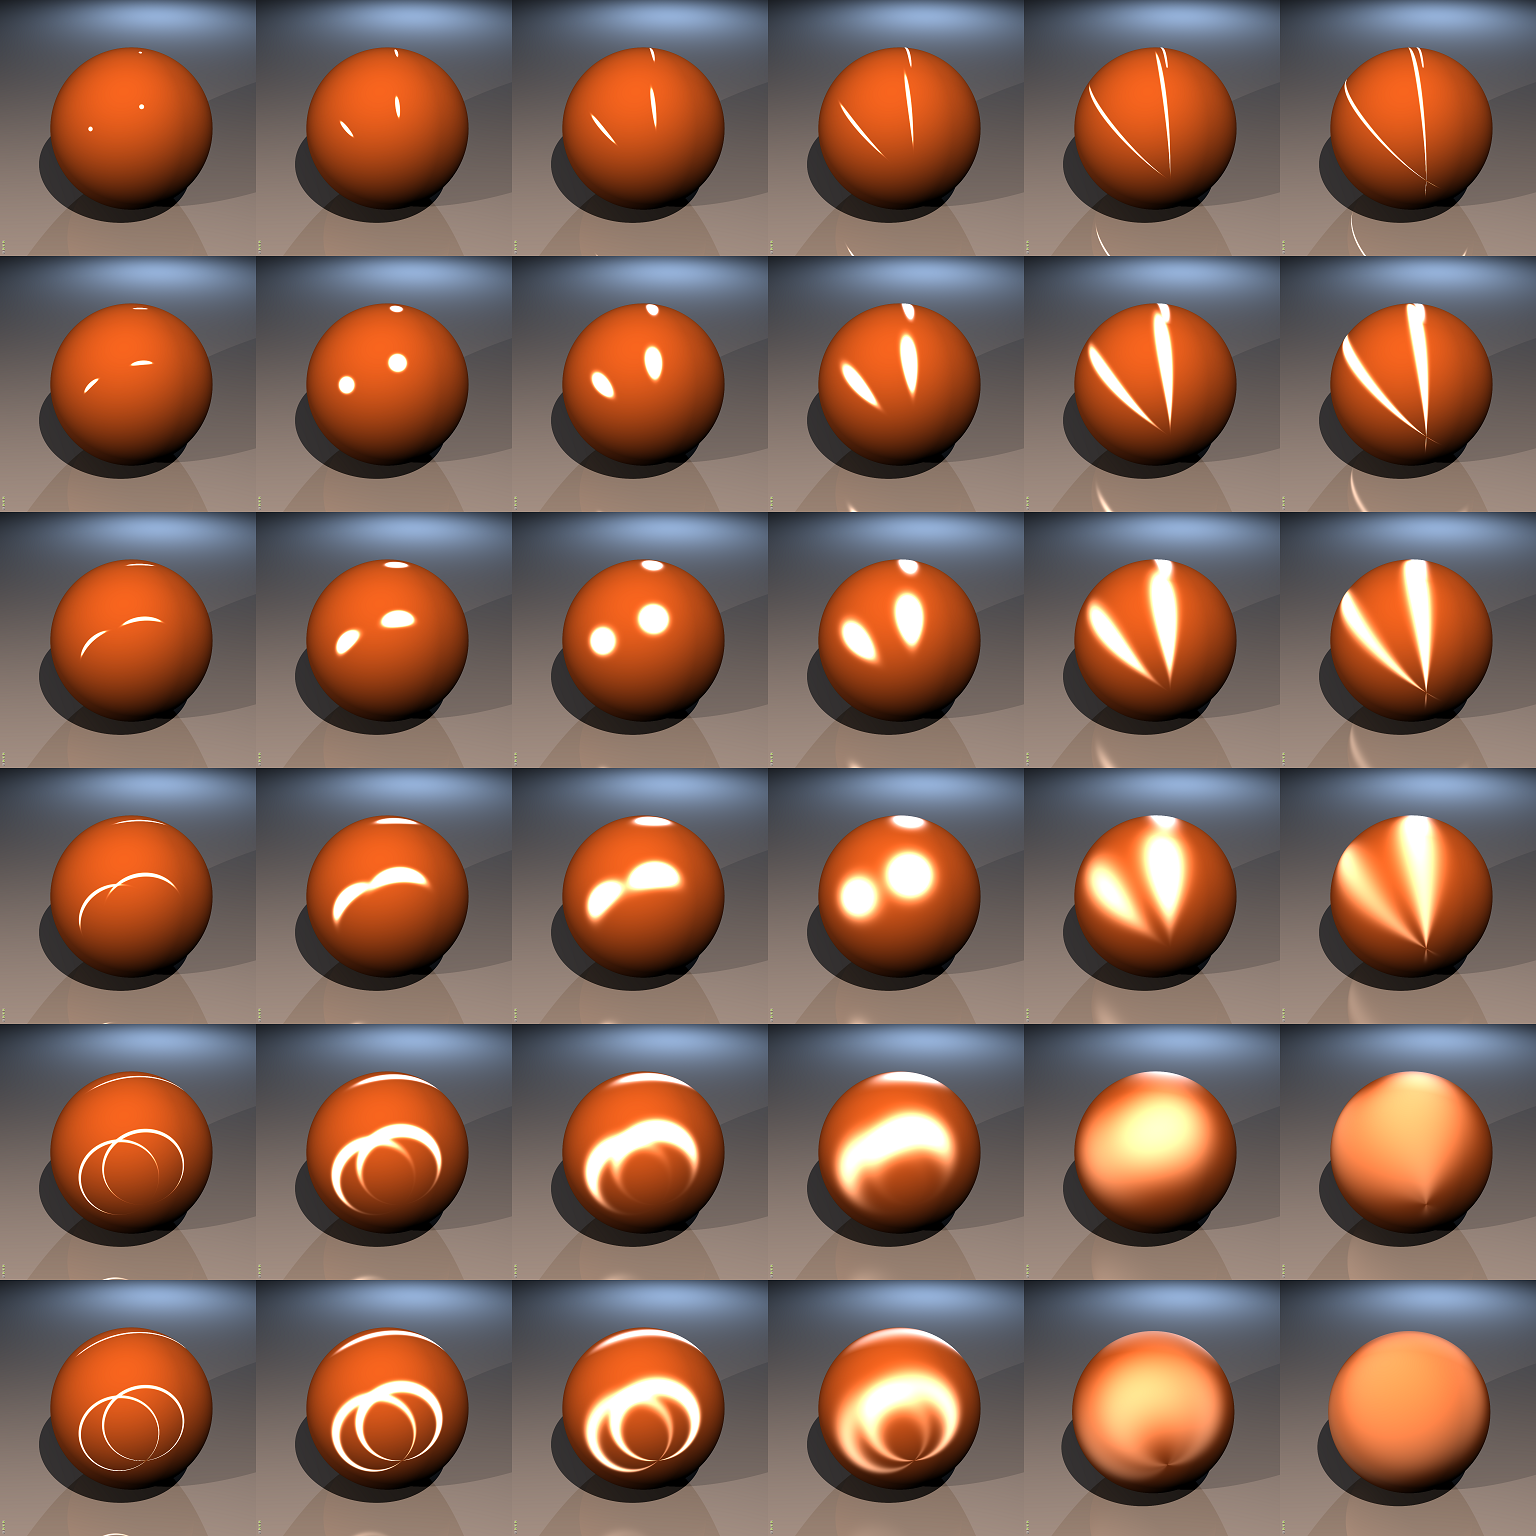
\includegraphics[height=\textheight]{../warduvcomplete.png}
\caption{Parameter $\alpha_x$, $\alpha_y$ from $0.01$ to $1.00$}
\end{figure}

\end{frame}



\subsection{Ashikhmin Shirley}
\begin{frame}[allowframebreaks]
\frametitle{Ashikhmin Shirley}
%TODO
\begin{itemize}
\item basierend auf [AS00]
\item theoretisches, auf Mikrofacetten basierendes Modell
\item simuliert anisotrope metallische Oberflächen
\end{itemize}

\begin{equation}
K_d = \frac{28 \rho_d}{23 \rho_s} (1 - \rho_s)\left(1-\left(1- \frac{\vec{N} \cdot \vec{L}}{2}\right)^5\right)\left(1-\left(1-\frac{\vec{N} \cdot \vec{L}}{2}\right)^5\right)
\end{equation}
\begin{equation}
K_s = \frac{\sqrt{(n_u+1)(n_v+1)}}{8\pi} \frac{((\vec{N} \cdot \vec{H})^{ \frac{n_u(\vec{H} \cdot \vec{U})^2 + n_v(\vec{H} \cdot \vec{V})^2}{1-(\vec{H} \cdot \vec{N})^2})}}{(\vec{H} \cdot \vec{L}) max((\vec{N} \cdot \vec{L}),(\vec{N} \cdot \vec{V}))} F(\vec{L} \cdot \vec{H})
\end{equation}

\framebreak
\begin{equation}
F(\vec{L} \cdot \vec{H}) = \rho_s + (1-\rho_s)(1-(\vec{L} \cdot \vec{H}))^5
\end{equation}

\begin{table}[H]
\begin{tabular}{| c | l |}
\hline
$n_u$ & Parameter : controls anisotropic behavior in $\vec{U}$ direction\\ \hline
$n_v$ & Parameter : controls anisotropic behavior in $\vec{V}$ direction\\ \hline
$\vec{U}$ & Tangent Vector to $\vec{N}$\\ \hline
$\vec{V}$ & Tangent Vector to $\vec{N}$, perpendicular to $\vec{U}$\\ \hline
\end{tabular}
\end{table}

\framebreak

\begin{figure}[H]
\centering

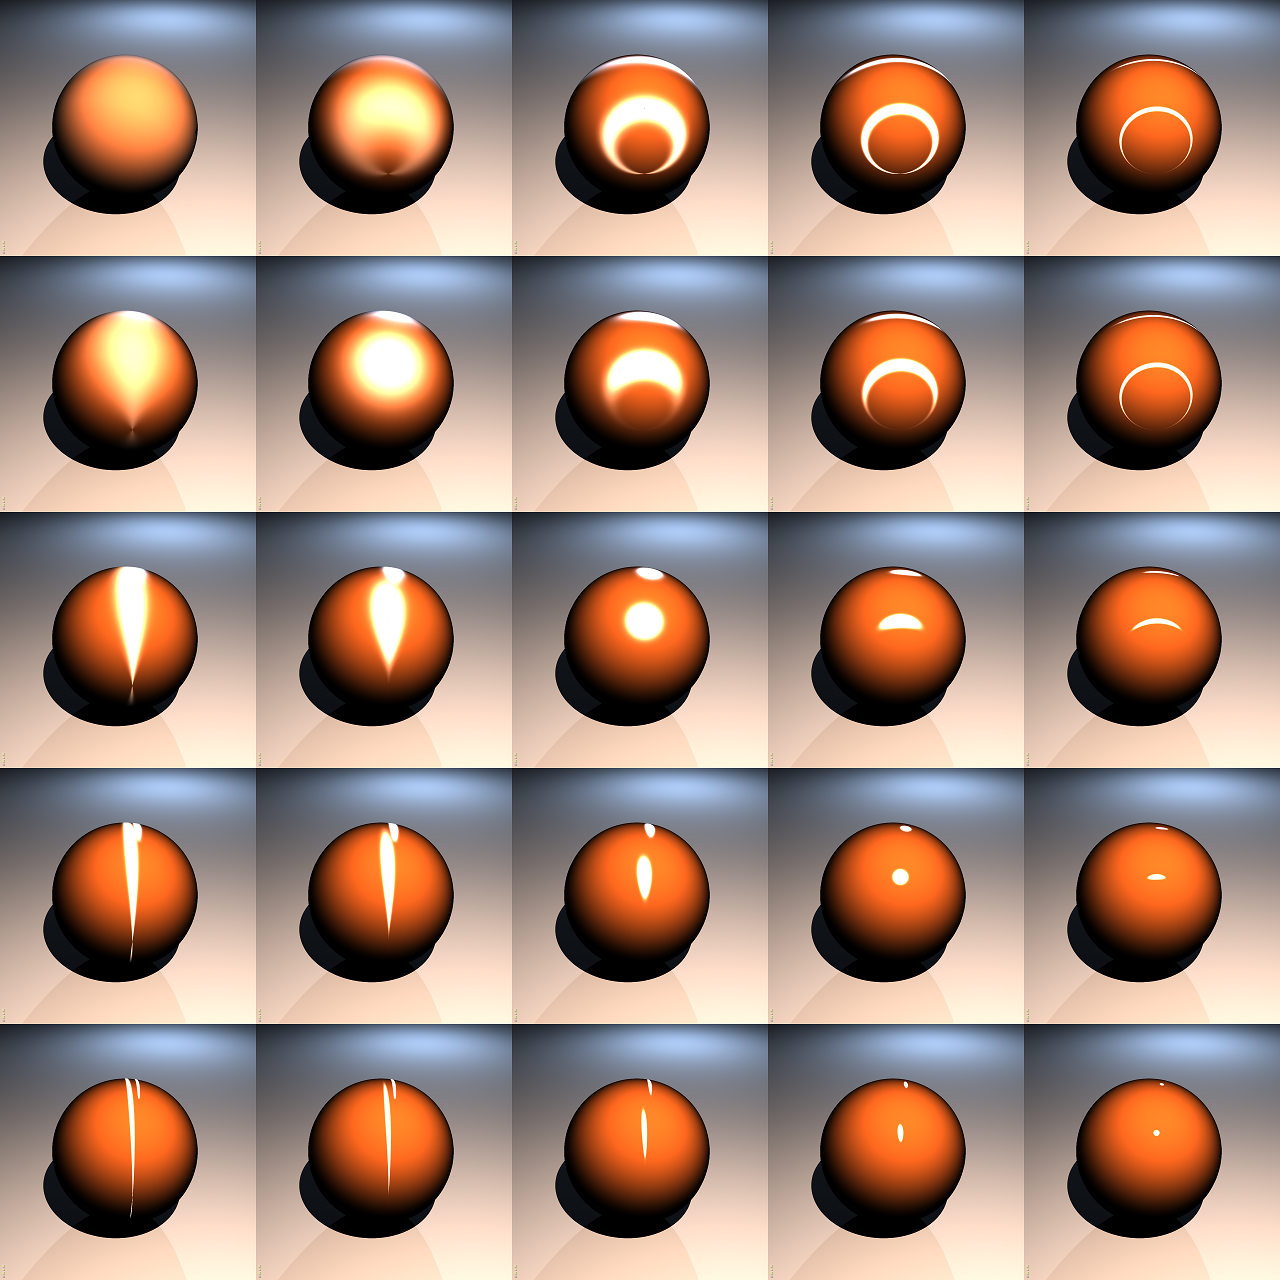
\includegraphics[height=0.8\textheight]{../ashuvcomplete.png}
\caption{Parameter $n_u$, $n_v$ from $1$ to $10000$}
\end{figure}

\framebreak

\begin{figure}[H]

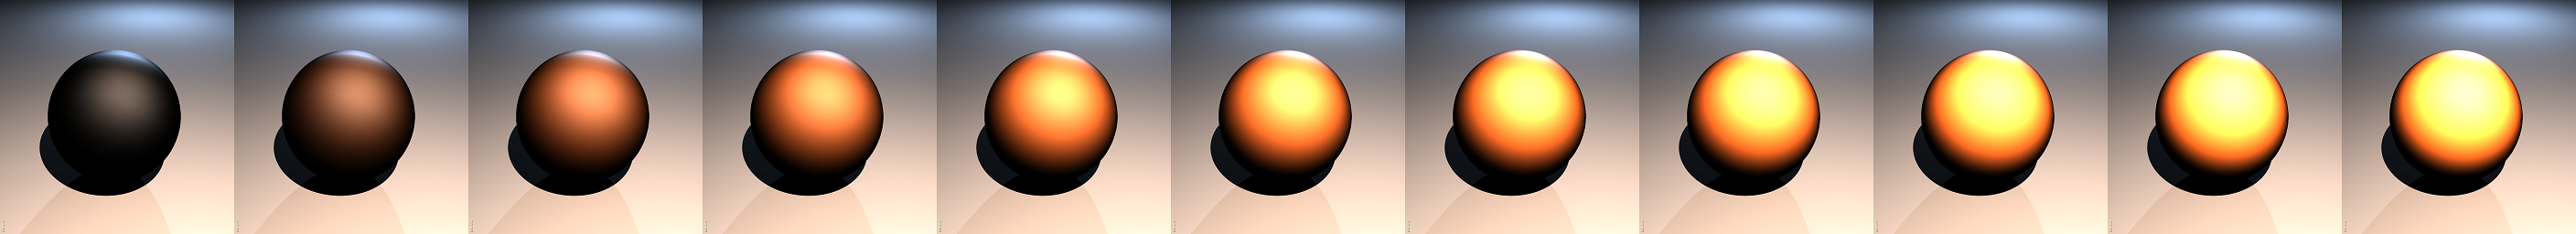
\includegraphics[width=\textwidth]{../ashdiffcomplete.png}
\caption{Parameter $\rho_d$ from $0.0$ to $1.0$}
\end{figure}

\begin{figure}[H]

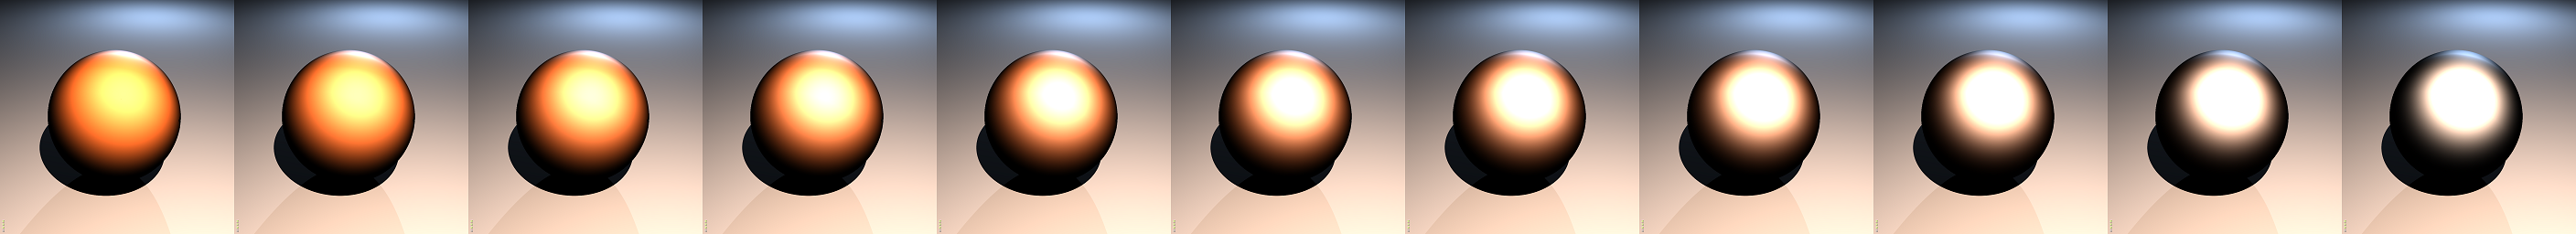
\includegraphics[width=\textwidth]{../ashspeccomplete.png}
\caption{Parameter $\rho_s$ from $0.0$ to $1.0$}
\end{figure}

\end{frame}



\subsection{Glas}
\begin{frame}[allowframebreaks]
\frametitle{Glas}
%TODO
\begin{itemize}
\item beschrieben als Dirac Delta in einer BSDF
\item simuliert durchsichtige Objekte
\end{itemize}

\begin{equation}
L_o(x,\vec{\omega_o})= \delta \cdot L_i(x,\vec{\omega_r}) + (1-\delta) L_i(x,\vec{\omega_t})
\end{equation}
\begin{equation}
\delta(\theta) = \delta_0 + (1-\delta_0)(1-cos\theta)^5
\end{equation}
\begin{equation}
\delta_0 = \left(\frac{n_t-1}{n_t+1}\right)^2
\end{equation}
\begin{table}[H]
\begin{tabular}{| c | l |}
\hline
$\delta$ & reflectivity of a dieletric\\ \hline
$\vec{\omega_r}$ & reflected view direction\\ \hline
$\vec{\omega_t}$ & transmitted view direction\\ \hline
$n_t$ & Parameter : refractive index of the surface\\ \hline
\end{tabular}
\end{table}

\framebreak

\begin{figure}[H]
\caption{Parameter $n_t$ from $1.0$ to $2.0$}
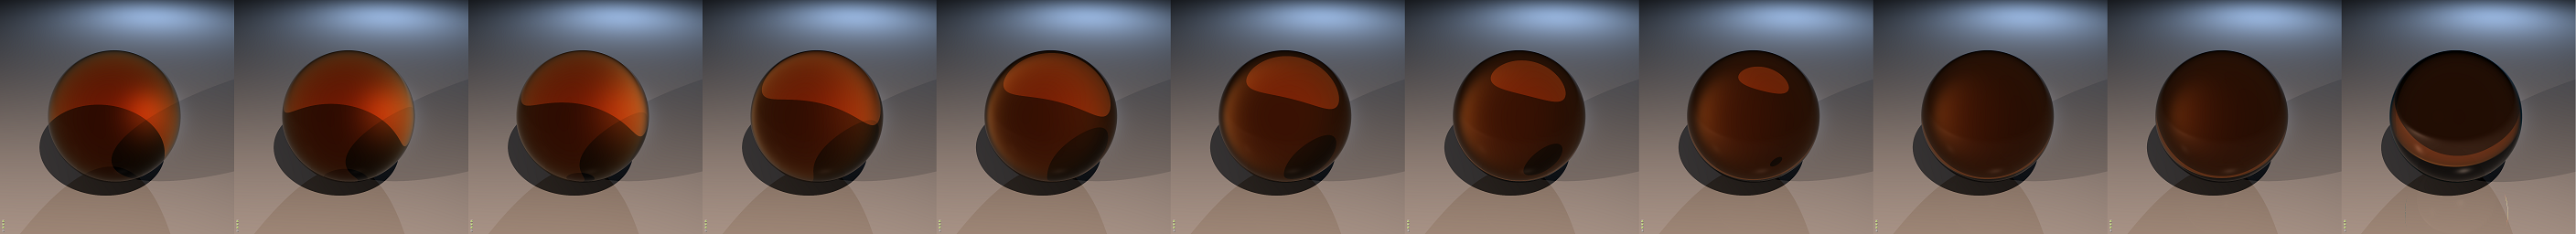
\includegraphics[width=\textwidth]{../glasscomplete.png}
\end{figure}

\end{frame}



\section{Ergebnisse}
\begin{frame}[allowframebreaks]
\frametitle{Ergebnisse}
\begin{center}
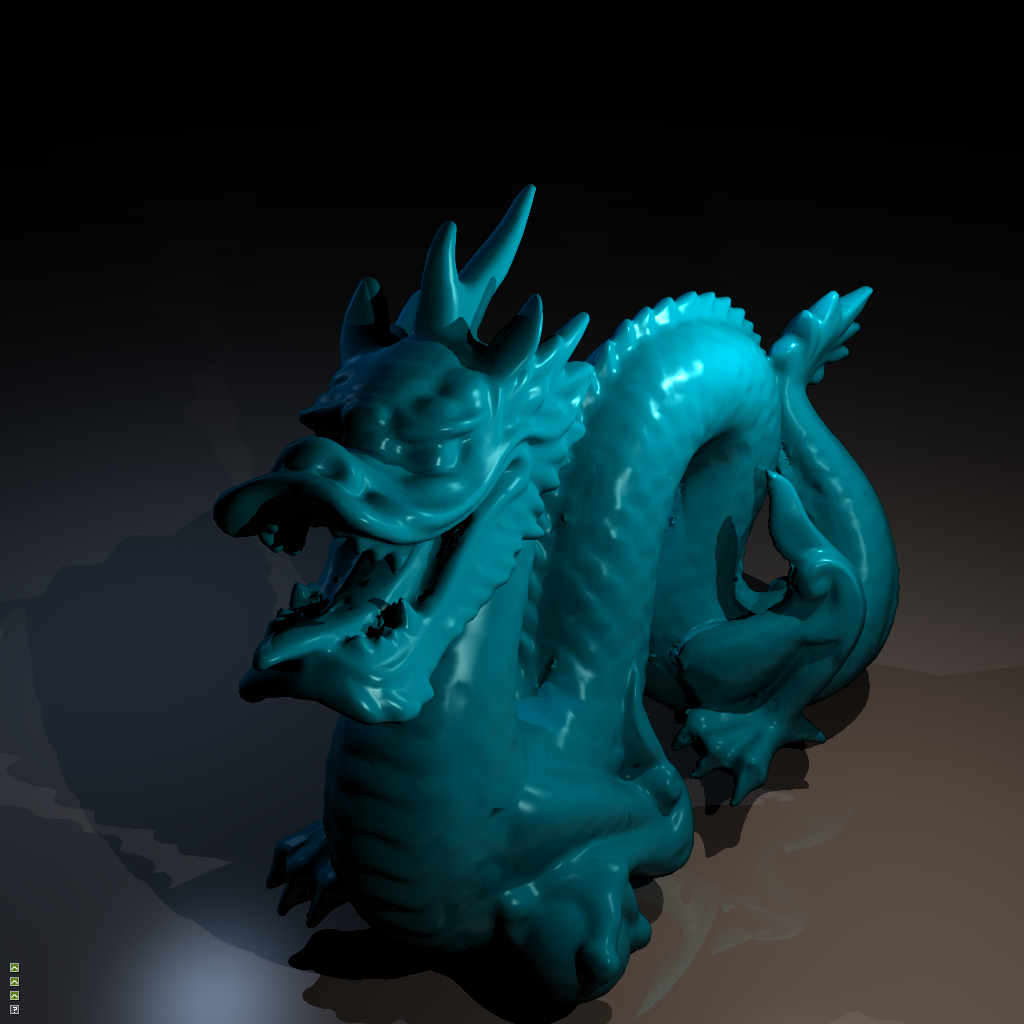
\includegraphics[width=0.6\linewidth]{../blueplastic}
\end{center}

\framebreak
\begin{center}
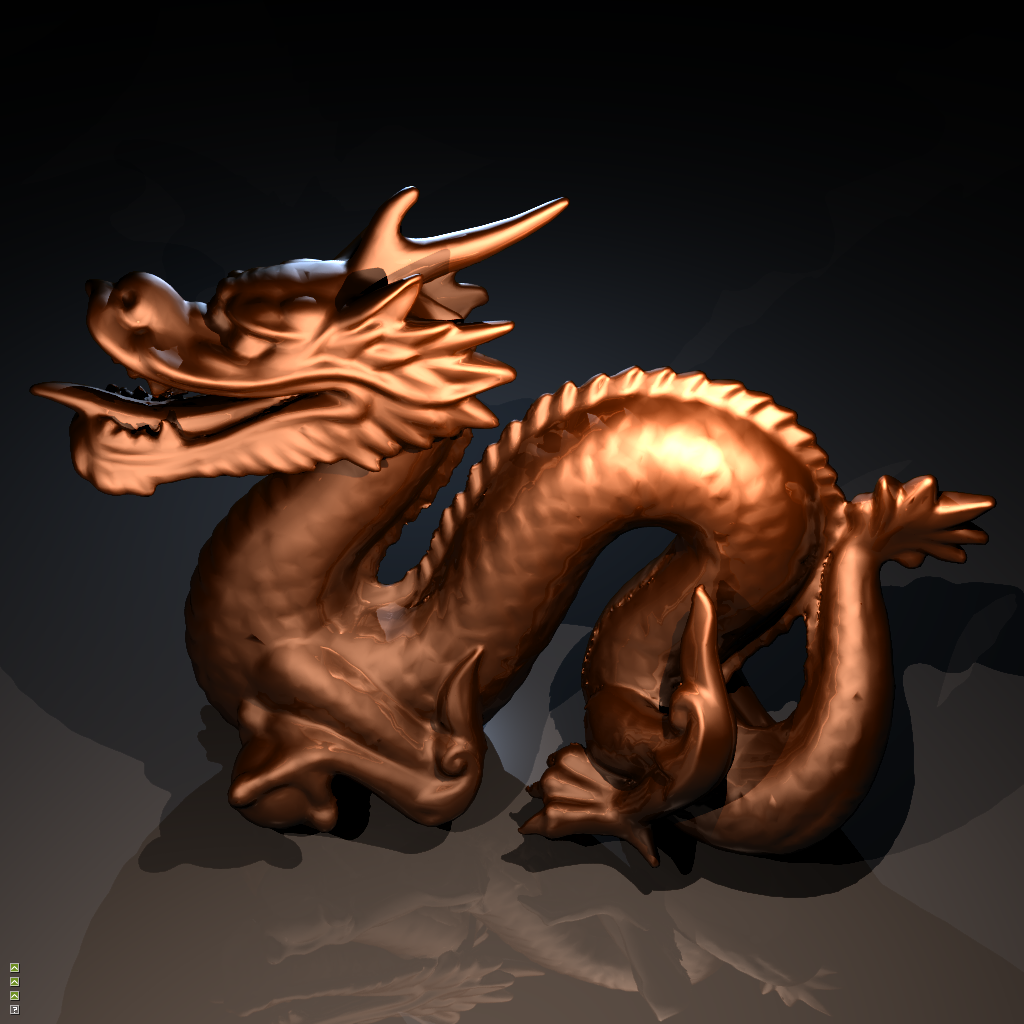
\includegraphics[width=0.6\linewidth]{../copperdragon}
\end{center}

\framebreak
\begin{center}
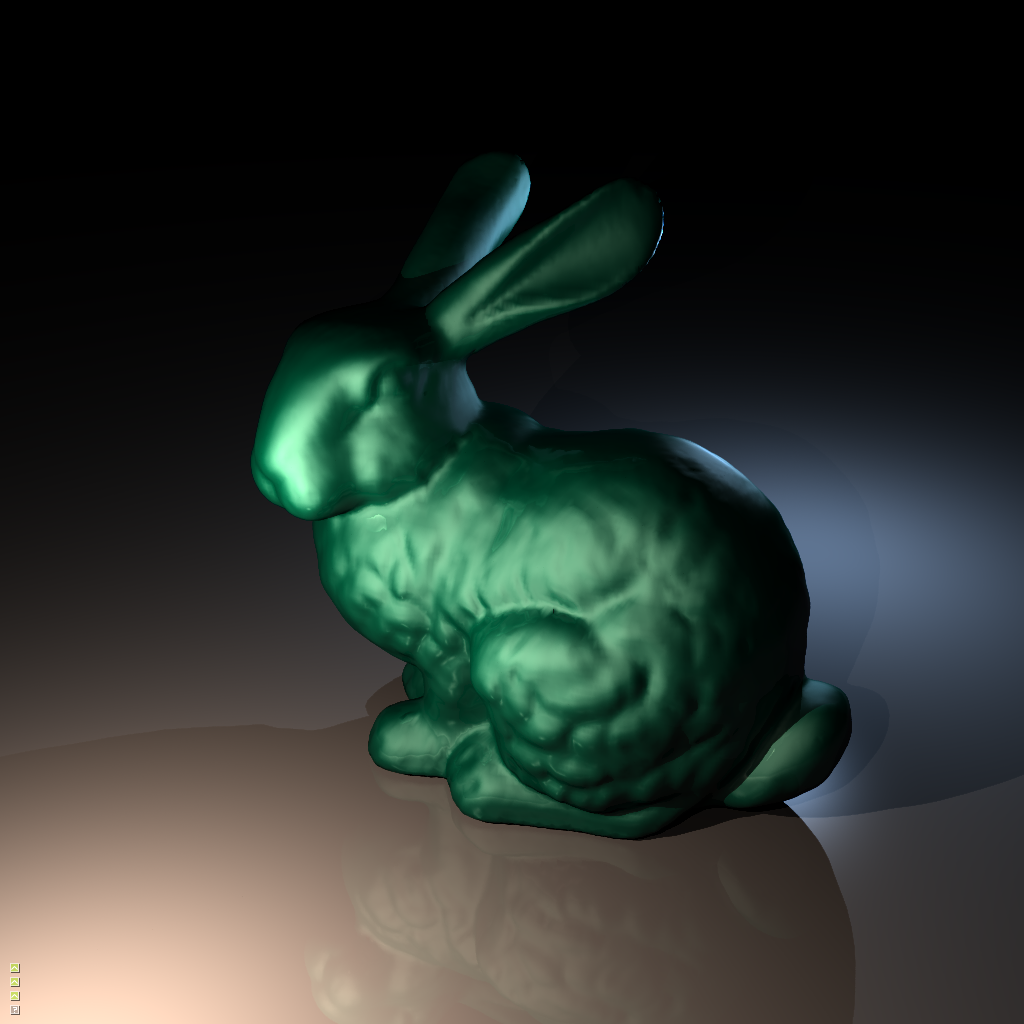
\includegraphics[width=0.6\linewidth]{../greenbunny}
\end{center}

\framebreak
\begin{center}
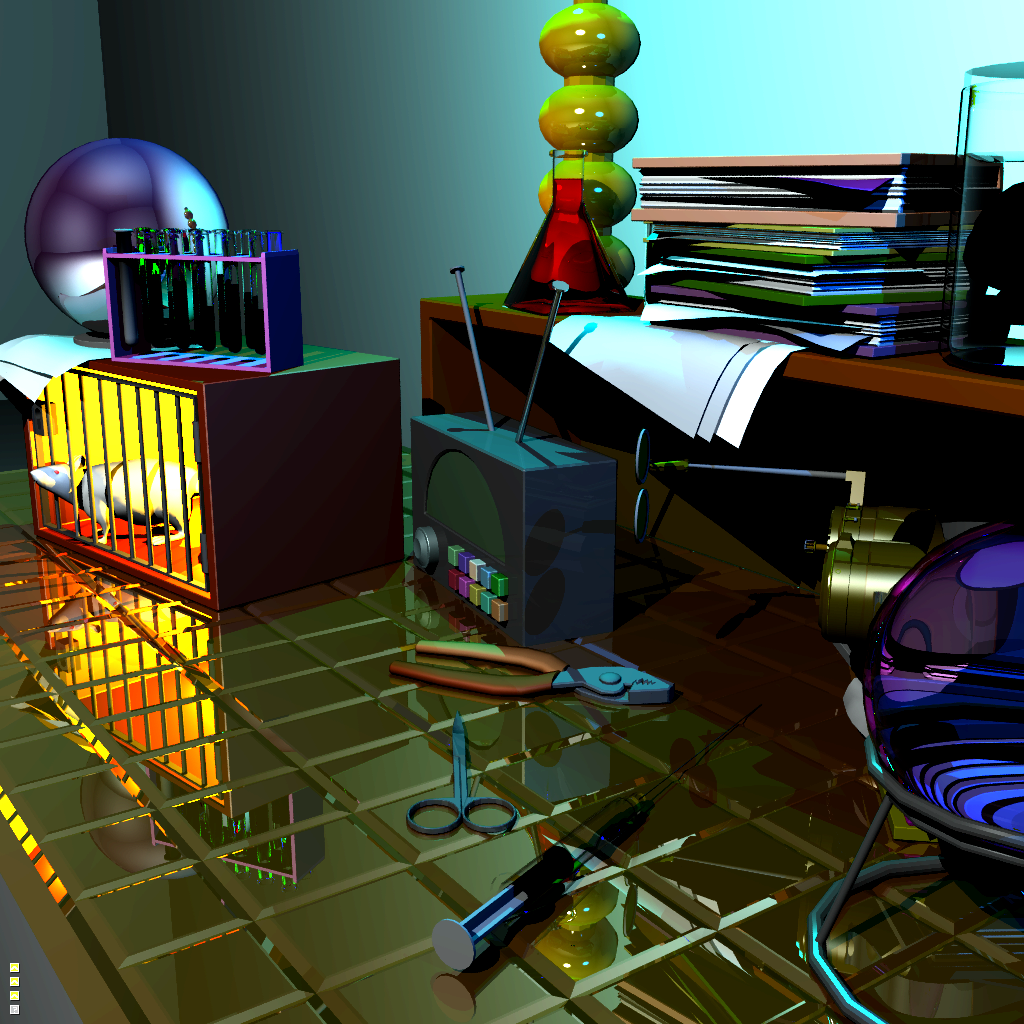
\includegraphics[width=0.95\linewidth]{../madlabcomplete_light}
\end{center}

\end{frame}



\section{Demo}
\begin{frame}
\frametitle{Demo}

\begin{center}
Wir beenden unsere Präsentation nun \\ mit einer live Demonstration unseres Raytracers.
\end{center}
 
\end{frame}


\end{document}